\documentclass[a4paper]{article}

\usepackage[hidelinks]{hyperref}
\usepackage{fullpage}
\usepackage{multirow}
\usepackage{graphicx}
\usepackage{mathtools}
\usepackage[english]{babel}
\usepackage[utf8]{inputenc}
\usepackage{fancyhdr}
\usepackage[left=1in,right=1in,top=1in,bottom=1in,headheight=8cm,headsep=0.5cm]{geometry}
\usepackage{changepage}
\usepackage{dingbat}
\usepackage{amsmath,mathpazo}
\usepackage[shortlabels]{enumitem}

\usepackage[dvipsnames]{xcolor}
\usepackage{tikz}
\usetikzlibrary{shapes}
\usetikzlibrary{calc}
\usepackage{anyfontsize}
\usepackage{sectsty}
\usepackage{setspace}
\usepackage{rotating}

\usepackage{appendix}
\usepackage{longtable}
\usepackage{array, booktabs}

\usepackage{fancyvrb} 
\usepackage[Export]{adjustbox}
\usepackage[listings]{tcolorbox}
\usepackage{lastpage}
\usepackage[lastpage,user]{zref}

\usepackage{float}
\usepackage{etoolbox}

\usepackage{tocloft}
\renewcommand{\cftsecleader}{\cftdotfill{\cftdotsep}} % Dots after section title
\renewcommand \thesection{\arabic{section}}
\renewcommand \thesubsection{\arabic{section}.\alph{subsection}} % Makes subsections alph

\usepackage[backend=biber,doi=false,isbn=false,url=false,eprint=false,annotation=false,alldates=year,useprefix=false,style=apa,natbib]{biblatex}
\usepackage{csquotes}
\usepackage{biblatex}
\bibliography{PCCA.bib}

\usepackage{titlesec}
\titleformat{\section}
{\normalfont\Large\bfseries}{\thesection}{1em}{}
\titleformat{\subsection}
{\normalfont\large\bfseries}{\thesubsection}{1em}{}
\definecolor{mygray}{gray}{0.9}

% changes footnote line length and thickness
\renewcommand{\footnoterule}{%
  \kern -3pt
  \hrule width 0.5\textwidth height 0.5pt
  \kern 2pt
}

\usepackage{titling}

\title{PCCA}
\author{Don Lim}
\date{\today}

\DeclareCiteCommand{\citetitleyear}
{\boolfalse{citetracker}%
  \boolfalse{pagetracker}}
{\ifciteindex
  {\indexfield{indextitle}}
  {}%
  \printfield[citetitle]{labeltitle}%
  \setunit{\addspace}%
  \printtext[parens]{%
    \usebibmacro{prenote}%
    \printfield{year}\printfield{extrayear}%
    \usebibmacro{postnote}}}
{\multicitedelim}
{}

\pagestyle{fancy}
\renewcommand{\headrulewidth}{0.2pt}
\fancyhf{}
\rhead{\emph{Survey Report}}
\lhead{Plains Cotton Cooperative Association}
\rfoot{\thepage\ of \zpageref{LastPage}}
% \lfoot{\today}

\definecolor{darkblue}{RGB}{20,20,220}
\hypersetup{
	colorlinks=true,
	linkcolor=darkblue,
	filecolor=darkblue,      
	urlcolor=darkblue,
	citecolor=darkblue,
}

\begin{document}

\pagestyle{empty}

\begin{tikzpicture}[remember picture,overlay]
	\fill[MidnightBlue] (current page.south west) rectangle (current page.north east);
	\begin{scope}
		\foreach \i in {2.5,...,22}
		{\node[rounded corners,MidnightBlue!50,draw,regular polygon,regular polygon sides=6, minimum size=\i cm,ultra thick] at ($(current page.west)+(2.5,-5)$) {} ;}
	\end{scope}
	\node[rounded corners,fill=MidnightBlue!60,text =MidnightBlue!5,regular polygon,regular polygon sides=6, minimum size=2.5 cm,inner sep=0,ultra thick] at ($(current page.west)+(2.5,-5)$) {};
	\foreach \i in {0.5,...,22}
	{\node[rounded corners,MidnightBlue!70,draw,regular polygon,regular polygon sides=6, minimum size=\i cm,ultra thick] at ($(current page.north west)+(2.5,0)$) {} ;}
	\foreach \i in {0.5,...,22}
	{\node[rounded corners,MidnightBlue!85,draw,regular polygon,regular polygon sides=6, minimum size=\i cm,ultra thick] at ($(current page.north east)+(0,-9.5)$) {} ;}
	\foreach \i in {12}
	{\node[fill = MidnightBlue
		,rounded corners,draw=MidnightBlue,regular polygon,regular polygon sides=6, minimum size=\i cm,ultra thick] at ($(current page.south east)+(-0.2,-0.45)$) {} ;}
	\foreach \i in {21,...,6}
	{\node[MidnightBlue!95,rounded corners,draw,regular polygon,regular polygon sides=6, minimum size=\i cm,ultra thick] at ($(current page.south east)+(-0.2,-0.45)$) {} ;}
	\node[left,MidnightBlue!5,minimum width=0.625*\paperwidth,minimum height=3cm, rounded corners] at ($(current page.north east)+(-1,-9.5)$){{\fontsize{25}{30} \selectfont \bfseries Plains Cotton Cooperative Association 2022}};
	\node[left,MidnightBlue!10,minimum width=0.625*\paperwidth,minimum height=2cm, rounded corners] at ($(current page.north east)+(3.25,-12)$){{\huge \textit{Survey Report}}};
	\node[left,MidnightBlue!10,minimum width=0.625*\paperwidth,minimum height=2cm, rounded corners] at ($(current page.north east)+(3.25,-14)$){{\Large \textit{}}};
	\node[right,MidnightBlue!5,minimum width=0.625*\paperwidth,minimum height=2cm, rounded corners] at ($(current page.north east)+(-9,-16)$){{\Large \textsc{Don Lim}}};
	\node[right,MidnightBlue!5,minimum width=0.625*\paperwidth,minimum height=2cm, rounded corners] at ($(current page.north east)+(-9.95,-17)$){{\Large \textsc{Landon Woods}}};
	\node[right,MidnightBlue!5,minimum width=0.625*\paperwidth,minimum height=2cm, rounded corners] at ($(current page.north east)+(-9.5,-18)$){{\Large \textsc{Steven Rios}}};
\end{tikzpicture}
\newpage
% \begin{titlingpage}
% 	\maketitle
% 	\begin{abstract}
		
% 	\end{abstract}
% 	Word count: 
% \end{titlingpage}
\thispagestyle{empty}


\noindent\begin{minipage}{0.5\textwidth}
	\raggedright
	\textbf{Texas Tech University} \\
	Department of Agriculture and Applied Economics \\
\end{minipage}%
\begin{minipage}{0.5\textwidth}
	\raggedleft
	Don Lim \\
	Landon Woods \\
	Steven Rios \\
	(806) \\
	Email:
\end{minipage}
\begin{center}
	\textbf{\large Memorandum}
\end{center}

\begin{flushleft}
	\today
\end{flushleft}
\begin{flalign*}
	& \text{TO: } & & \text{Ms. Jayci Bishop} & \\
	& \text{FROM: } & & \text{Don Lim} & \\
	& & & \text{Landon Woods} & \\
	& & & \text{Steven Rios} & \\
	& \text{SUBJECT: } & & \text{Summary of Understanding and Background Information for the PCCA Case} & 
\end{flalign*}

\singlespacing

This report seeks to use information gathered by questionnaire survey data to address future development of PCCA. During a meeting with the PCCA staff, concerns were expressed over the changing preferences of existing members. Additionally, newer members, who may be part of the younger generation, may have different preferences and valuations regarding cooperatives. Additionally, they may have different skills and have obtained more formal education compared to the older generation. By adding new members, PCCA provides a greater range and volume of quality products to buyers which strengthens its market position. We aim to evaluate how members feel about PCCA's communication and customer service, evaluate how members value being part of the cooperative, determine member knowledge of PCCA marketing options, and inquire how members receive information related to farming and the cotton industry.

The questionnaire is directed at PCCA members and will be asked to PCCA members online. The main goal, then, is to answer the following questions:

\begin{enumerate}[noitemsep]
	\item Are the PCCA members satisfied with the overall customer support and information that PCCA provides?
	\item Where do PCCA members get their information related to farming and cotton growing, and how can PCCA provide better information?
	\item How effective is PCCA at communicating with its members through social media, their website, and their app?
\end{enumerate}
 
In order to retain existing members and attract new ones, the value, information, and customer service PCCA provides must be more attractive than the alternative cooperatives and the option of selling individually on the market. The questionnaire and the following analysis should give a better understanding of how satisfied existing members are with the services PCCA provides, and formulate a strategic plan going forward. 

\newpage

\thispagestyle{empty}
\pagenumbering{gobble}
\tableofcontents

\newpage
\pagestyle{fancy}
\pagenumbering{arabic}
\setcounter{page}{1}

\doublespacing

\section{Problem statement}

Farming is largely a generational industry. With more of the older farmers are retiring and younger incoming members, there could be different attitudes and shifts in opinions about the value and role of cooperatives. We want to determine if younger members value the cooperative differently than their parent's generation. Since younger farmers are more technologically adept, we should determine how the sources of information differ from generation to generation and how that becomes a determinant if they choose membership. 

In order to retain existing members and attract new ones, the value, information, and customer service PCCA provides must be better than the alternative cooperatives and the option of selling individually on the market. The survey and the following analysis should give a better understanding of how satisfied existing members are with the services PCCA provides.

The questionnaire is directed at PCCA members and will be asked online. The goal, then, is to answer the following questions:

\begin{enumerate}[noitemsep]
	\item Are the PCCA members satisfied with the overall customer support and information that PCCA provides?
	\item Where do PCCA members get their information related to farming and cotton growing, and how can PCCA provide better information?
	\item How effective is PCCA at communicating with its members through social media, their website, and their app?
\end{enumerate}

\section{Objectives}

This report seeks to use information gathered by survey data in order to address the future development of PCCA. During a meeting with the PCCA staff, concerns were expressed over the changing preferences of existing and potentially new members. In order to make recommendations, the following information must be acquired:
\begin{enumerate}[noitemsep]
	\item Evaluate how members feel about PCCA's communication and customer service
	\item Evaluate how members value being part of the cooperative
	\item Determine member knowledge of PCCA marketing options
	\item Inquire how members receive information related to farming and the cotton industry
\end{enumerate}

\section{Historical overview}
This section borrows heavily from \citet{HistoryPlainsCotton2004}.\footnote{The source is cited from \citet{pedersonInternationalDirectoryCompany2004}, however, we were unable to track down a copy of the text.} The Plains Cotton Cooperative Association (PCCA) was formed in 1953. A group of cotton farmers, with a combined fund of \$12,000 sought to create an outlet to obtain the best price in cotton trade. Today, with an average of 2-3 million bales handled annually, representing 15-20\% of the US market cotton cap, PCCA is one of the largest cotton handlers in the US.

In order to fund this growth, a record of constant innovation can be seen through the decades. In 1960, PCCA developed the high volume instrument (HVI) classing system. This system allowed samples from each bale to be tested into a classing office for a more consistent product. In 1973, PCCA assisted in the formation of the American Cotton Growers Association (ACG), a farmer-owned cooperative, that also served west Texas cotton producers. In 1975, under PCCA management, ACG began construction of a cotton textile mill in Littlefield, Texas. The following year, the mill went into production. The mill then applied state-of-the-art technology to produce optimum yarn strength, allowing ACG to manufacture heavyweight denim exclusively for Levi Strauss \& Company. 

\subsection{Technology}

During the 1970s and 1980s, PCCA transferred its system of cotton trading to an electronic platform. In 1975, the first electronic marketing system for cotton was created, TELCOT. The technology allowed buyers and sellers to trade at a centralized location. In 1985, PCCA formed TELMARK, Inc. to provide TELCOT services to independent ginning outfits and cotton producers in Texas and Oklahoma. PCCA also introduced the Online Gin Bookkeeping system (OGB) that replaced the paper bookkeeping with an electronic system designed for cotton gins. In 1989, PCCA supported electronic warehouse receipts and electronic title system technologies, which allowed cotton to be traded more efficiently electronically. As a result of all these technological advancements, on February 1989, TELCOT processed the trade of 385,599 bales of cotton in a single day. In 2000, PCCA released The Seam online trading system, which is a nationwide business software that allows product listings outside of cotton.

In 2003, PCCA launched its Member Access and later, the myPCCA app. PCCA's Member Access system allows members to view the relevant informant regarding gin, ticket information, and statements freely. Members can sign up for text alerts related to class information, scale ticket information, and futures prices (goods include cotton, corn, feeder cattle, wheat, live cattle, and soybean) 

\subsection{Marketing programs}

In 1987, PCCA purchased the denim mill from ACG. The purchase brought more than \$100 million in revenue to PCCA members in west Texas and southwestern Oklahoma. This vertical integration from the cotton farms to the textile market undoubtedly further garnered membership into the cooperative. At the same time of this acquisition, PCCA introduced pool marketing to its members as an alternative to regular trade and crop contracting. While pool marketing was already available to ACG members, this now allowed PCCA members to combine cotton from various producers and to sell as a group. The program also provided baling, storage, and stock management, allowing producers to focus entirely on cotton production. Producers can choose the growing season and types of cotton to grow. Another program that was introduced was the Mill Option Program, which allowed members to obtain earnings from the profits of the mill. In 1988, all of these services were extended to the region of south Texas. 

Thus far, PCCA offers four marketing methods to sell cotton:
\begin{enumerate}[noitemsep]
	\item The Seam
	\item Forward marketing
	\item Pool marketing
	\item PCCA direct
\end{enumerate}

As mentioned in the earlier section, The Seam online trading system was implemented in 2000. This allows for anonymous trading and guaranteed bale quality and payments. In addition, The Seam provides access to more cotton trading opportunities through more cotton buyers, more competitive prices, and more efficient transference of cotton from the field to the merchant or the mill. Another marketing program PCCA provides is bale forward contracting. This contract can be formed post-harvest (sold to PCCA) or pre-harvest (sold as individual contracts or pooled). Forward contracting allows cotton to be sold at a certain and concrete price, which reduced price risk. Pooled contracting could achieve long-term above average returns. The dividend is paid out at the end of the ear. The last marketing option is PCCA direct. This option allows members to sell directly to PCCA rather than to other buyers.

\subsection{Uncertain times}

Starting in the late 1990s, the US cotton industry, including PCCA, experienced times of great uncertainty. With foreign competition in cotton, cotton apparel, and textiles increasing, the supply of cotton and cotton-related goods increased while the price decreased. To add to the uncertainty, Levi Strauss informed PCCA and other textile producers that it could no longer guarantee volume purchases of fabric. The mill PCCA purchased from ACG produced nearly 36 million yards of heavyweight denim, nearly all of it sold to Levi Strauss. PCCA would have to find additional buyers of denim. 

However, there was a silver lining from the uncertain market. More farmers were taking advantage of the pool marketing option to reduce the amount of risk they faced. This also created another opportunity for PCCA due to the changing circumstances and preferences of its members. As more members used pool marketing, fewer used the TELCOT system. On May 2000, PCCA formed a joint venture to transfer TELCOT to an internet platform for trading cotton and cotton product and services online. This new company, named The Seam, was created in November and operational in December. Since the late 1990s, the textile industry experienced heavy losses in employment \citep{nelsonhodgesEmploymentTextileApparel2006}. In 2001, PCCA reported its first net loss since 1985. However, as PCCA continued to operate and develop denim styles with new dye methods and finishes, as well as new stretch Lycra and cotton blend fabric, the denim market improved. 

\section{Literature review}

The cooperative form of business was formed initially in New York. The first cooperative was a dairy association that began in the mid-1800s. It was created to combat the monopsony power of privately held milk-processing plants \citep{porterEconomicEfficiencyCooperatives1987,erdmanRevolvingFinanceAgricultural1965}. One definition of a cooperative, as \citet{kollerCooperativesCapitalisticEconomy1947} puts it, can be "a form of business organization---an economic entity---owned and controlled by its member patrons for the rendering of services for their mutual benefit as patrons." However, while cooperatives depend on organizational growth, member heterogeneity may cause a decline in market position, if agricultural cooperatives do not adapt quickly and successfully \citep{cookCooperativeLifeCycle2009}. In other words, if the preferences of the cooperative's members are too heterogeneous, this increases the probability of organizational degeneration \citep{hansmannOwnershipEnterprise2000,chaddadUnderstandingNewCooperative2004,iliopoulosInfluenceCostsAgribusiness2009}. Applying this literature to PCCA, PCCA recognizes that with incoming members belonging to the newer generation, there could be substantial member heterogeneity, that is, differences in interests, needs, and preferences, of members. 

\citet{hohlerDimensionsMemberHeterogeneity2018} conceptualize member heterogeneity into three categories:
\begin{enumerate}[noitemsep]
	\item Farm-level heterogeneity
	\begin{itemize}[noitemsep]
		\item Size-related: differences in farm size
		\item Spatial: different geographical locations of cooperative's members. This may include different production conditions as well as different cultures
	\end{itemize}
	\item Member-level heterogeneity
	\begin{itemize}[noitemsep]
		\item Personal: age, experience, education, income, decision-making behavior
		\item Temporal: variance in the planned and duration of memberships
		\item Risk references: differences in investment constraints
		\item Contractual: differences in relationships between members and cooperatives
		\item Participatory: differences in members' commitment to participate in a cooperative's governance
		\item Motivational: differences in members' valuation of the benefits of membership
	\end{itemize}
	\item Product-related heterogeneity: differences in the kind, quality, or amount of products delivered to the cooperative
\end{enumerate}

For the purposes of our investigation into PCCA, we are primarily concerned with member-level heterogeneity, particularly related to personal, participatory, and motivational heterogeneity. We aim to find the causes for the differences in preferences, customer satisfaction, and cooperative valuation between members. This is to develop a strategic plan to foster continued PCCA growth. As \citet{nilssonAreLargeComplex2012} note, there is a "multiplicator effect" -- the sense that members are able to provide the cooperative with financial support that, in turn, builds social capital, and this builds further human capital (a build-up of mutual trust with increased interactions and communication). The model \citet{munchAssessingValueCooperative2021} provide suggest that members value cooperative ownership proportionally with more years of education and farming experience. \citet{kleinDeterminantsCooperativePatronage1997} find older farmers tend to patronize cooperatives and large farms tend to patronize cooperatives. Larger firms also do a greater share of their business with cooperatives than do smaller firms. It would be interesting to note if this is true for PCCA members. Additionally, farmers that believe cooperatives offer innovative products and services are more likely to patronize them. 

One possible mechanism to foster human capital is social media. \citet{culnanHowLargeCompanies2010} examine how large U.S. companies can use Twitter and other social media to communicate with their customers. They found that simply creating an online presence is insufficient to gain business value from social media. Instead, successful implementation requires three elements: mindful adoption, community building, and absorptive capacity. Likewise, regarding cooperatives, \citet{ciruela-lorenzoDigitalizationAgriCooperativesSmart2020} write, 
\begin{quote}
	Maintaining inertia and concentrating on traditional activity can no longer be considered a viable option. It is necessary to diversify the activity, innovate and collaborate with others, incorporating talent and using new technologies in order to better compete in a sustainable way.
\end{quote} Indeed, cooperatives can adopt the same guidelines in order to extract similar business value as firms from social media. One of the reasons for using social media is to retain existing members and to attract new ones. 

Member responses from the questionnaire would also help us evaluate their preferences and desires regarding PCCA. \citet{pinsonneaultSurveyResearchMethodology1993} define a survey as a "means for gathering information about the characteristics, actions, or opinions of a large group of people" (p. 77). Additionally, \citet{grovesSurveyMethodology2009} notes, "surveys are ubiquitous tools of management to improve the performance of their organizations" (p. 5). Poor data quality is very common when constructing surveys. Matters such as irrelevant questions, questions with an overwhelming bias, and a small sample size result in inaccurate data for the surveys. Constructing a survey that limits these errors will provide better data. Irrelevant questions will waste the survey taker's time and not result in data that pertains to the study, questions with an overwhelming bias will result in data that is altered to fit a certain narrative that could be inaccurate, and a small sample size would not represent all potentially diverse opinions. Data analysis is crucial when deciding what decisions need to be made that work in the best interests of the company. Close-ended questions help determine what the population's exact opinions are on certain topics with multiple options whereas open-ended questions allow for better insight on specific matters that the population has thoughts on. Filtering results by cross-tabulating subgroups and analyzing the data from different groups is also beneficial and will help in having the data be easier to interpret. 

\section{Data}

The data used for this research study was provided through an online questionnaire. The sample group is PCCA members. The questionnaire included a mix of multiple-choice, yes-no questions, and open-ended questions; it asked members to rank on a 6-point scale the satisfaction with PCCA communication, information services, customer service, and marketing options. The survey also included questions involving the respondent's knowledge on PCCA marketing methods (pool marketing, The Seam, PCCA direct, and forward contracting). The respondents could choose between "No knowledge," "Some knowledge," or "Extensive knowledge." We code "Strongly disagree" as 1, "Disagree" as 2, "Somewhat disagree" as 3, "Somewhat agree" as 4, "Agree" as 5, and "Strongly agree" as 6. We code "No knowledge" as 1, "Some knowledge" as 2, and "Extensive knowledge" as 3. Dummy variables were created for members who use social media, traditional media, interpersonal communication, industry organization, and using the cooperative. Within social media, dummy variables were created for members who use new media, Facebook, Twitter, Instagram, YouTube, Snapchat, and TikTok. More open-ended questions were asked to respondents related the perceived value of PCCA, the reasons behind joining PCCA, and concerns regarding PCCA and its future.\footnote{The full survey can be viewed \href{https://www.sogosurvey.com/preview1.aspx?k=YsQQXRYSsQW&status=preview}{here}.} 3,969 PCCA members were identified and 3,852 email surveys were successfully delivered. 354 surveys were returned for a response rate of 8.8 percent. 

\section{Data visualizations}
\subsection{Entire sample}

For now, let us view the general trends in from the PCCA survey report.

\noindent\begin{minipage}{0.5\textwidth}
	\begin{figure}[H]
		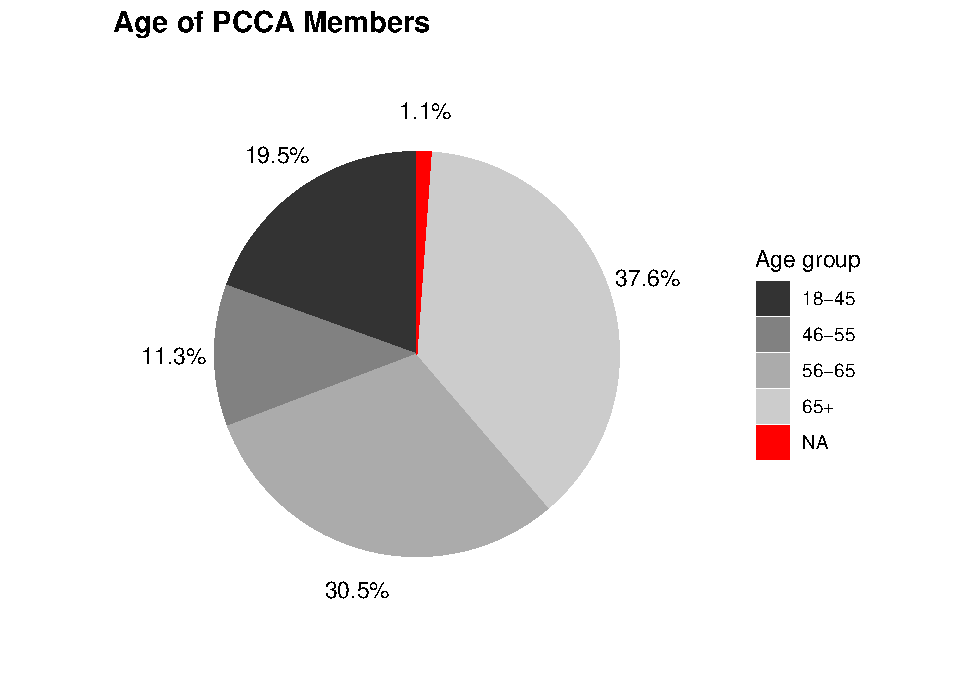
\includegraphics[scale=0.6]{survey/pcca_survey_files/figure-latex/age-all-1.pdf}
	\end{figure} 
\end{minipage}%
\begin{minipage}{0.5\textwidth}
	\begin{figure}[H]
		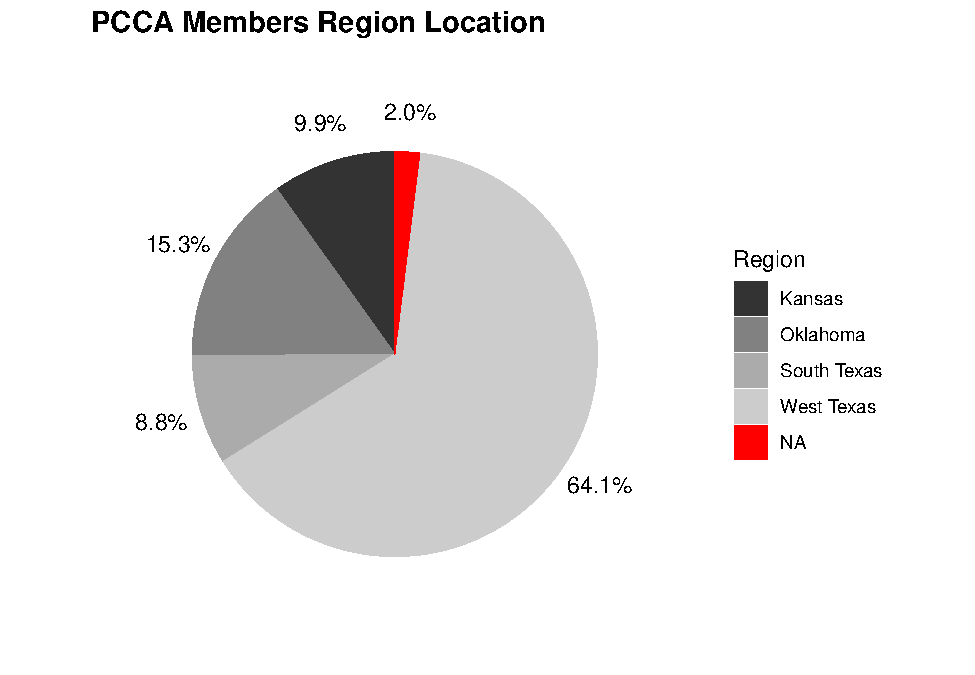
\includegraphics[scale=0.6]{survey/pcca_survey_files/figure-latex/region-all-1.pdf}
	\end{figure}
\end{minipage}

From here, we see the majority of the respondents are age 56 and over and reside in south and west Texas.

\begin{minipage}{0.5\textwidth}
	\begin{figure}[H]
		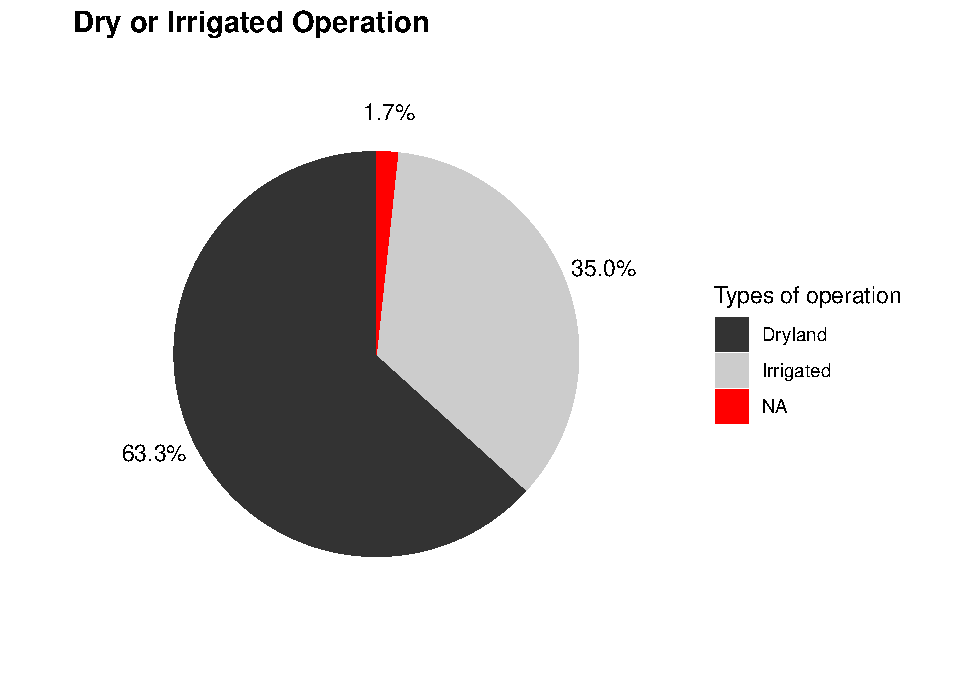
\includegraphics[scale=0.6]{survey/pcca_survey_files/figure-latex/operation-all-1.pdf}
	\end{figure}
\end{minipage}%
\begin{minipage}{0.5\textwidth}
	\begin{figure}[H]
		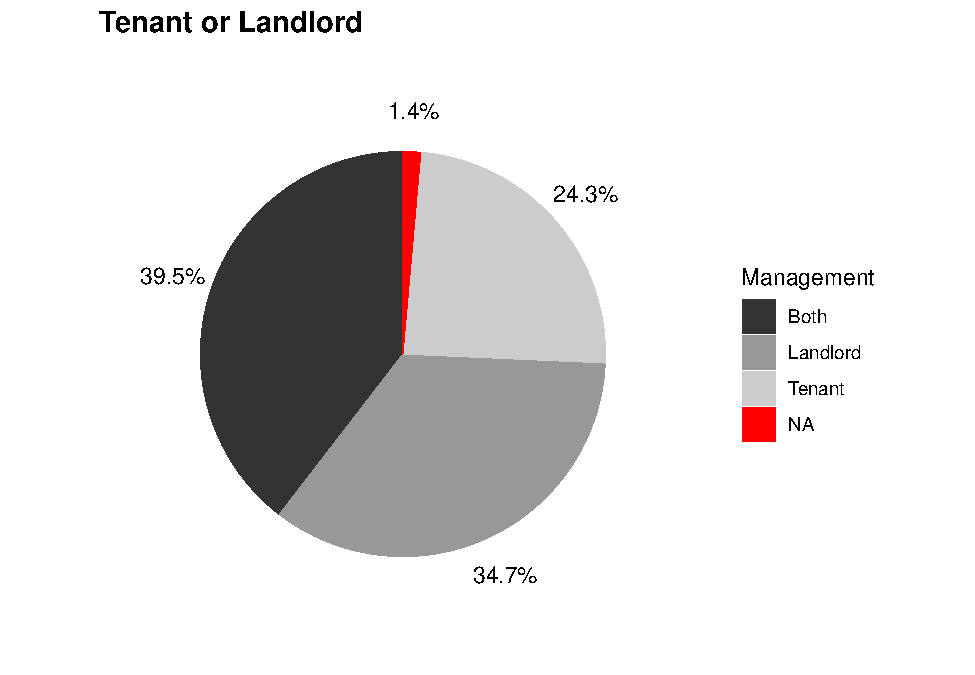
\includegraphics[scale=0.6]{survey/pcca_survey_files/figure-latex/tenant-all-1.pdf}
	\end{figure}
\end{minipage}

Most respondents operate under dryland and there is about an even split among landlords and tenants. 

\begin{minipage}{0.5\textwidth}
	\begin{figure}[H]
		\centering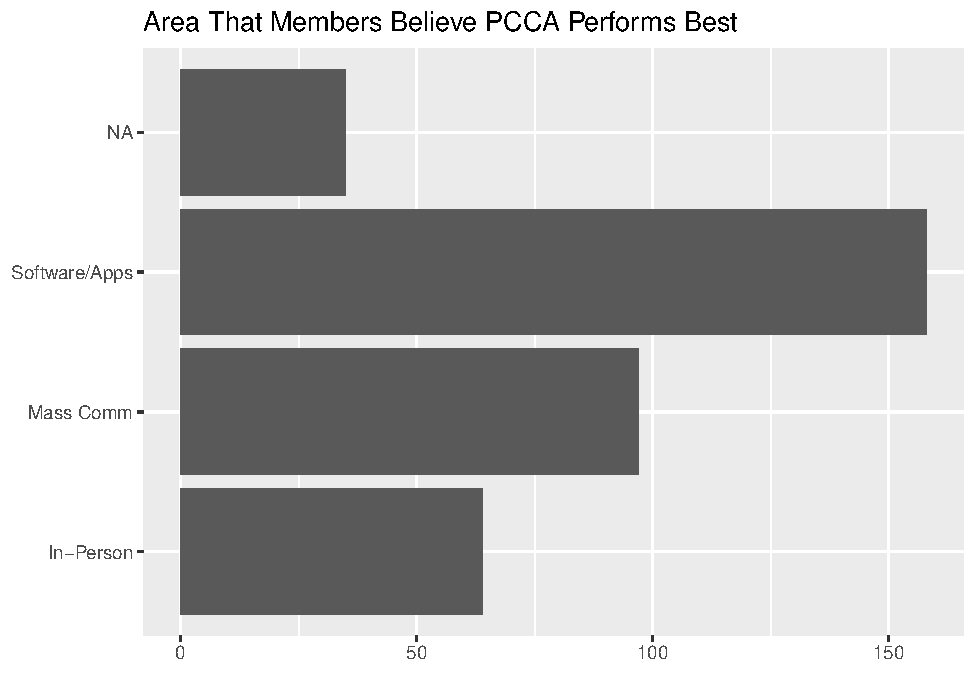
\includegraphics[scale=0.45]{survey/pcca_survey_files/figure-latex/best-all-1.pdf}
	\end{figure}
\end{minipage}%
\begin{minipage}{0.5\textwidth}
	\begin{figure}[H]
		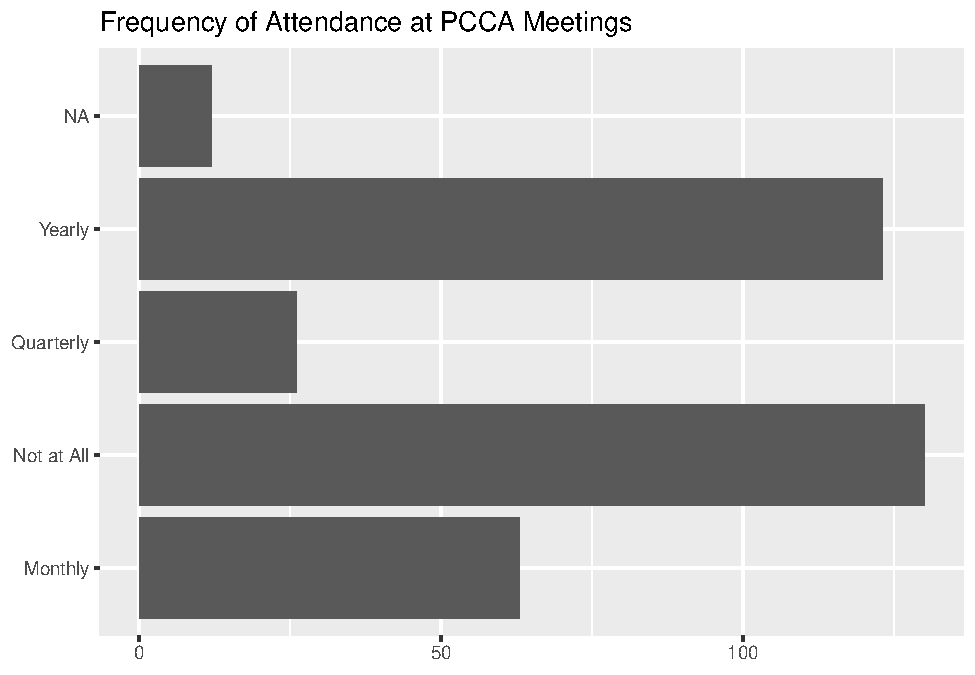
\includegraphics[scale=0.45]{survey/pcca_survey_files/figure-latex/meetings-all-1.pdf}
	\end{figure}
\end{minipage}

For the most part, PCCA members believe that PCCA performs best with their software and app development. However, given that the respondents from the survey seem more educated and comfortable with technology, it seems this sample may over-represent PCCA members who use the software and app features more frequently.

\subsection{Younger vs older generation}
However, since we also want to see if there are any potential differences between the younger and older generations, we should split up the data and separately visualize each group. For paper, we consider the younger generation as the age bracket of 18-45. There are 69 respondents for the younger generation. The older generation is considered age 56-65 and 65+. There are 241 respondents for the older generation. For the next few figures, the younger generation will be visualized on the and the older will be on the right. \\

\noindent\begin{minipage}{0.5\textwidth}
	\centering\textbf{Younger}
	\begin{figure}[H]
		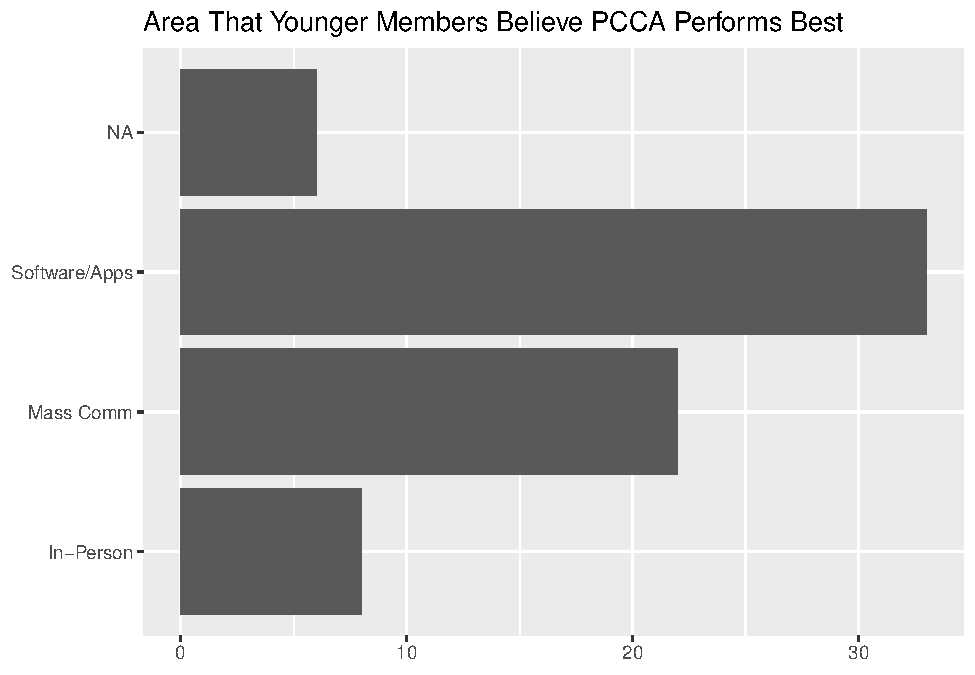
\includegraphics[scale=0.5]{survey/pcca_survey_files/figure-latex/best-young-1.pdf}
	\end{figure}
\end{minipage}%
\begin{minipage}{0.5\textwidth}
	\centering\textbf{Older}
	\begin{figure}[H]
		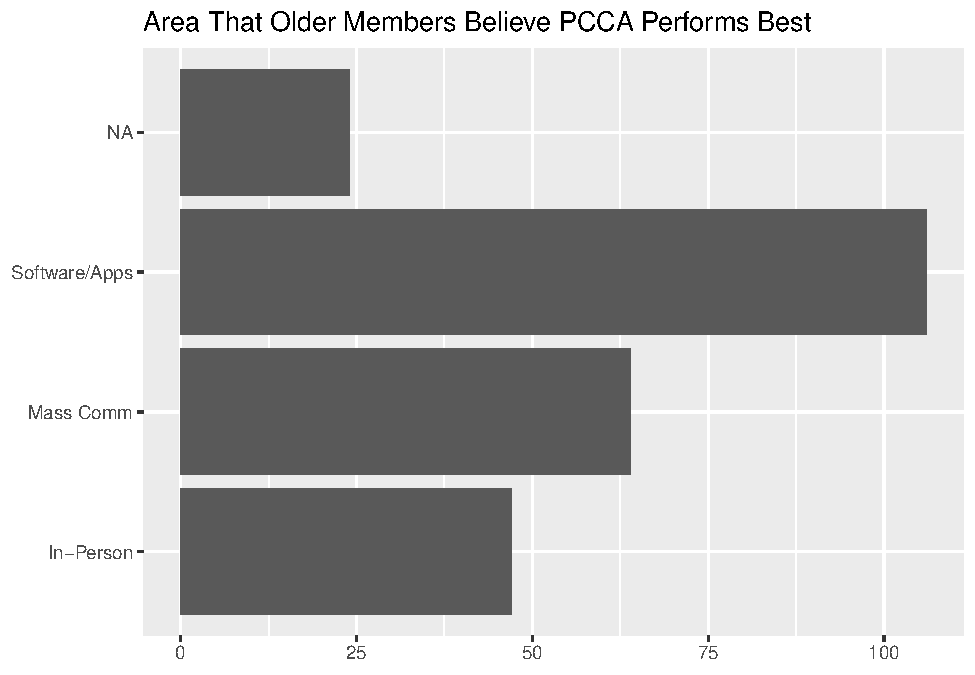
\includegraphics[scale=0.5]{survey/pcca_survey_files/figure-latex/best-old-1.pdf}
	\end{figure}
\end{minipage}

There is seemingly no difference between the younger and older generation in how they perceive the area that PCCA performs best.

\noindent\begin{minipage}{0.5\textwidth}
	\begin{figure}[H]
		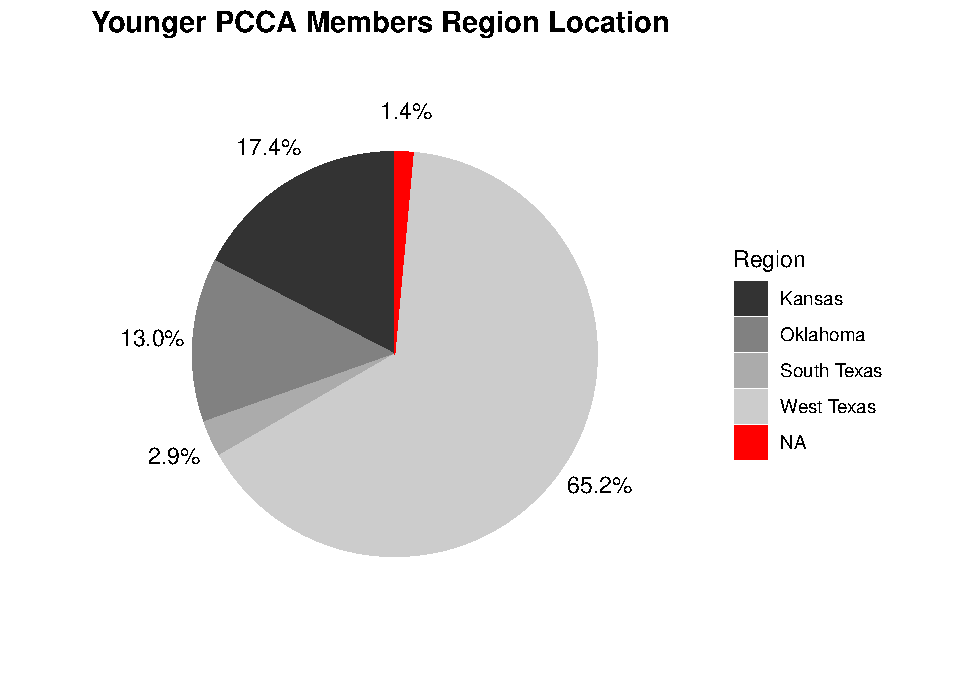
\includegraphics[scale=0.5]{survey/pcca_survey_files/figure-latex/region-young-1.pdf}
	\end{figure}
\end{minipage}%
\begin{minipage}{0.5\textwidth}
	\begin{figure}[H]
		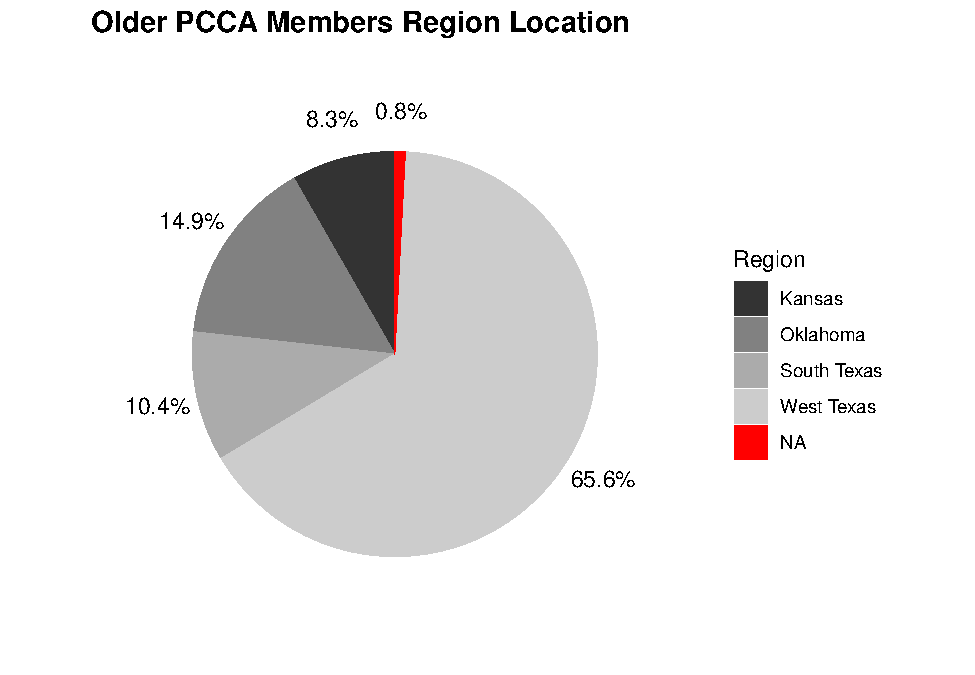
\includegraphics[scale=0.5]{survey/pcca_survey_files/figure-latex/region-old-1.pdf}
	\end{figure}
\end{minipage}

Kansas members seem to make up a greater proportion of younger PCCA membership compared to the older generation. However, it would be too much of an extrapolation to make this conclusion with this dataset given that we only have 69 observations out of the nearly 4,000 PCCA members. Further analysis is required to confirm if there are indeed greater younger Kansas farmers joining PCCA.

\noindent\begin{minipage}{0.5\textwidth}
	\begin{figure}[H]
		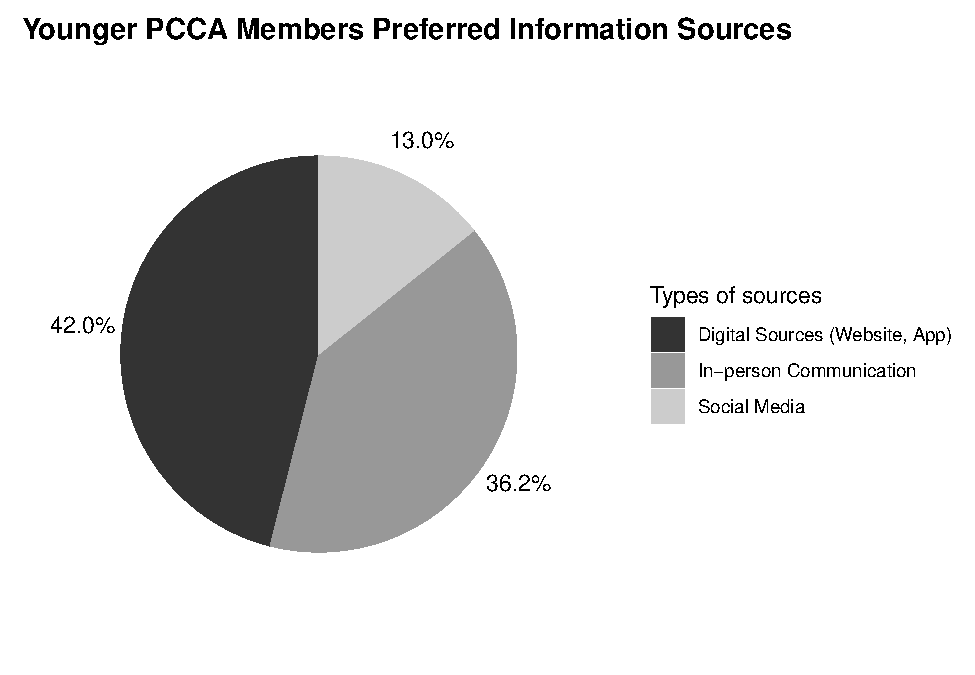
\includegraphics[scale=0.5]{survey/pcca_survey_files/figure-latex/information-young-1.pdf}
	\end{figure}
\end{minipage}%
\begin{minipage}{0.5\textwidth}
	\begin{figure}[H]
		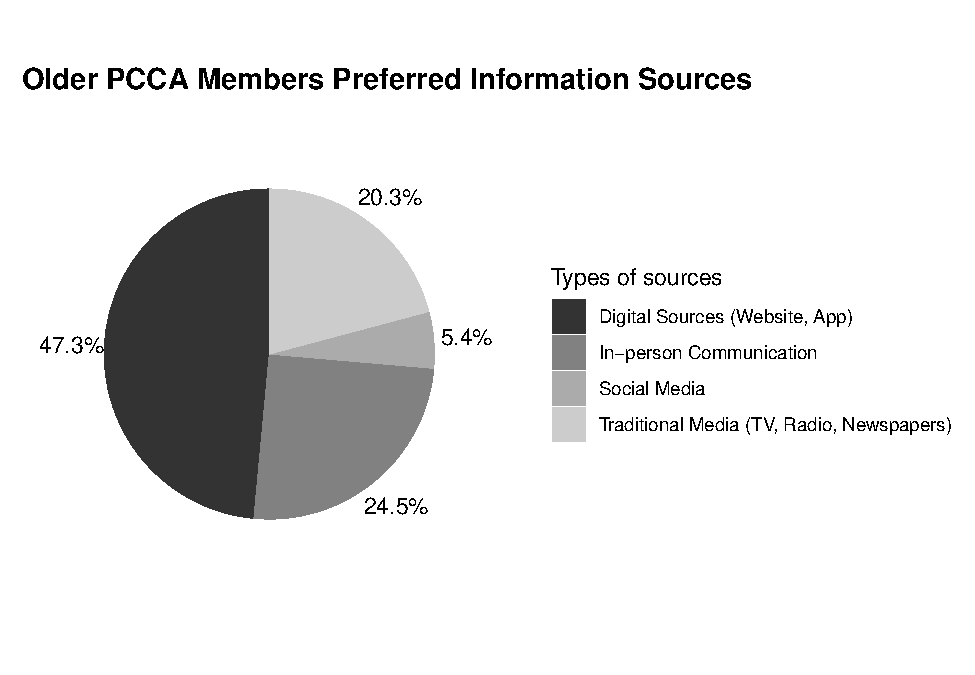
\includegraphics[scale=0.5]{survey/pcca_survey_files/figure-latex/information-old-1.pdf}
	\end{figure}
\end{minipage}

Unsurprisingly, while traditional media makes up 20.3 percent of the older generation's preferred information sources, it is completely absent from the younger generation. Moving forward, if PCCA still publishes traditional media, it would seem plausible to phase out those traditional media and to replace it with either digital sources, in-person communication, or social media.

\begin{table}[H]
	\caption{Self-reported Knowledge of Marketing Methods}
	\centering\begin{tabular}{l|llll}
		& Marketing Pool & The Seam & PCCA Direct & Forward Contracting \\
		\hline \hline
	Total & 2.174 (0.0319) & 1.735 (0.036) & 1.527 (0.0311) & 1.626 (0.0324) \\
	Younger & 2.203 (0.0639) & 1.927 (0.0725) & 1.536 (0.060) & 1.768 (0.0658) \\
	Older & 2.151 (0.0395) & 1.662 (0.0446) & 1.520 (0.0397) & 1.567 (0.0390)
	\end{tabular}
\end{table}

With further tests (see appendix), we find that there is a significant difference between the self-reported knowledge of younger and older generations for The Seam and forward contracting methods. The younger generation, on average, report themselves as being more knowledgeable on both methods. This makes sense since the marketing pool is the oldest method offered by PCCA. Some of the older members may have simply stuck to this method rather than explore any of the new offerings available. The younger generation, more experiment-bound, may have sought to explore other marketing options. For both younger and older PCCA members, it is evident that because the marketing pool method is the most popular, it is also the one that members feel like they are more knowledgeable about. 

\section{Statistical method}

For our model, let us attempt to predict the satisfaction PCCA members feel given how the member feels about the accessability, responsiveness, and courteousness of PCCA service. The model is given by:

\begin{align}
	Y_{i}=X'\beta+\epsilon_{i}
\end{align}

Expanding the model, we can estimate the parameters via ordinary least square (OLS) regression:
\begin{align}
	Y_{i}=\beta_{0}+\beta_{1}(accessible)+\beta_{2}(responsive)+\beta_{3}(courteous)+\epsilon_{i}
\end{align}

Where $Y_{i}$ is the satisfaction PCCA members report they have with PCCA. In the second model, let us include all the explanatory variables as the first \emph{and} include how knowledgeable the members are about the four marketing programs: pool marketing, The Seam, PCCA direct, and forward contracting.

\begin{equation}
	\begin{split}
		Y_{i}=\beta_{0}+\beta_{1}(accessible)+\beta_{2}(responsive)+\beta_{3}(courteous)+\beta_{4}(pool)+\beta_{5}(seam) \\ +\beta_{6}(direct)+\beta_{7}(forward)+\epsilon_{i}
	\end{split}
\end{equation}

This would, in effect, capture both how PCCA members perceive how accessible, responsive, and courteous they believe PCCA to be \emph{and} how knowledge affects their satisfaction with PCCA overall.


\section{Results and discussion}

\begin{singlespace}
	\begin{table}[H] \centering 
		\caption{Model 1} 
		\label{} 
	  \begin{tabular}{@{\extracolsep{5pt}}lc} 
	  \\[-1.8ex]\hline 
	  \hline \\[-1.8ex] 
	   & \multicolumn{1}{c}{\textit{Dependent variable:}} \\ 
	  \cline{2-2} 
	  \\[-1.8ex] & satisfaction \\ 
	  \hline \\[-1.8ex] 
	   accessible & 0.266$^{**}$ \\ 
		& (0.107) \\ 
		& \\ 
	   responsive & 0.452$^{***}$ \\ 
		& (0.128) \\ 
		& \\ 
	   courteous & 0.107 \\ 
		& (0.107) \\ 
		& \\ 
	   Constant & 0.369 \\ 
		& (0.357) \\ 
		& \\ 
	  \hline \\[-1.8ex] 
	  Observations & 329 \\ 
	  R$^{2}$ & 0.317 \\ 
	  Adjusted R$^{2}$ & 0.310 \\ 
	  Residual Std. Error & 1.059 (df = 325) \\ 
	  F Statistic & 50.194$^{***}$ (df = 3; 325) \\ 
	  \hline 
	  \hline \\[-1.8ex] 
	  \textit{Note:}  & \multicolumn{1}{r}{$^{*}$p$<$0.1; $^{**}$p$<$0.05; $^{***}$p$<$0.01} \\ 
	  \end{tabular} 
	\end{table}
\end{singlespace}

From our first model, we estimate, with a somewhat unsurprising result, that PCCA member perception of the accessibility and responsiveness of PCCA significantly influences their overall satisfaction with PCCA. If we, however, cluster around the younger and older generations, we find that none of the factors are significant for the younger generation; the overall effect is mainly driven by the older generation. This could be in part due to the larger observation size of the older generation since the magnitude between both generations are the same but the standard errors are much larger for the younger generation.

For the second model, the results are:

\begin{singlespace}
	\begin{table}[H] \centering 
		\caption{Model 2} 
		\label{} 
	  \begin{tabular}{@{\extracolsep{5pt}}lc} 
	  \\[-1.8ex]\hline 
	  \hline \\[-1.8ex] 
	   & \multicolumn{1}{c}{\textit{Dependent variable:}} \\ 
	  \cline{2-2} 
	  \\[-1.8ex] & satisfaction \\ 
	  \hline \\[-1.8ex] 
	   accessible & 0.293$^{***}$ \\ 
		& (0.106) \\ 
		& \\ 
	   responsive & 0.378$^{***}$ \\ 
		& (0.129) \\ 
		& \\ 
	   courteous & 0.168 \\ 
		& (0.107) \\ 
		& \\ 
	   `marketing pool` & 0.005 \\ 
		& (0.119) \\ 
		& \\ 
	   `the seam` & $-$0.242$^{**}$ \\ 
		& (0.117) \\ 
		& \\ 
	   `pcca direct` & 0.281$^{**}$ \\ 
		& (0.115) \\ 
		& \\ 
	   `forward contracting` & $-$0.110 \\ 
		& (0.126) \\ 
		& \\ 
	   Constant & 0.452 \\ 
		& (0.415) \\ 
		& \\ 
	  \hline \\[-1.8ex] 
	  Observations & 311 \\ 
	  R$^{2}$ & 0.369 \\ 
	  Adjusted R$^{2}$ & 0.354 \\ 
	  Residual Std. Error & 1.024 (df = 303) \\ 
	  F Statistic & 25.267$^{***}$ (df = 7; 303) \\ 
	  \hline 
	  \hline \\[-1.8ex] 
	  \textit{Note:}  & \multicolumn{1}{r}{$^{*}$p$<$0.1; $^{**}$p$<$0.05; $^{***}$p$<$0.01} \\ 
	  \end{tabular} 
	\end{table} 
\end{singlespace}

From the results, the magnitudes and significance are similar to the first model, however, we notice that the more educated about The Seam, the \emph{less} satisfaction they report towards PCCA overall. This is a particularly confusing finding and may warrant further investigation. 

\subsection{Probit model}

Given that there were some puzzling aspects in model two, let us attempt to use a probit model in order to model dichotomous outcome variables. Given that respondents were able to choose the satisfaction of PCCA information with a slider from 1 to 6, with 1 indicating complete dissatisfaction and 6 indicating complete satisfaction, we will code scores of 4 and above to indicate a satisfied member in order to create the binary dependent variable. The model is

\begin{align}
	P(Y_{i}=1)=X'\beta+\epsilon_{i}
\end{align}

\begin{singlespace}
	\begin{table}[H] \centering 
		\caption{} 
		\label{} 
	  \begin{tabular}{@{\extracolsep{5pt}}lc} 
	  \\[-1.8ex]\hline 
	  \hline \\[-1.8ex] 
	   & \multicolumn{1}{c}{\textit{Dependent variable:}} \\ 
	  \cline{2-2} 
	  \\[-1.8ex] & satisfaction (0 or 1) \\ 
	  \hline \\[-1.8ex] 
	   accessible & 0.514$^{**}$ \\ 
		& (0.256) \\ 
		& \\ 
	   responsive & 0.673$^{**}$ \\ 
		& (0.313) \\ 
		& \\ 
	   courteous & 0.279 \\ 
		& (0.291) \\ 
		& \\ 
	   `marketing pool` & $-$0.173 \\ 
		& (0.329) \\ 
		& \\ 
	   `the seam` & $-$0.669$^{**}$ \\ 
		& (0.321) \\ 
		& \\ 
	   `pcca direct` & 0.602$^{*}$ \\ 
		& (0.319) \\ 
		& \\ 
	   `forward contracting` & 0.143 \\ 
		& (0.335) \\ 
		& \\ 
	   Constant & $-$5.137$^{***}$ \\ 
		& (1.260) \\ 
		& \\ 
	  \hline \\[-1.8ex] 
	  Observations & 311 \\ 
	  Log Likelihood & $-$123.808 \\ 
	  Akaike Inf. Crit. & 263.615 \\ 
	  \hline 
	  \hline \\[-1.8ex] 
	  \textit{Note:}  & \multicolumn{1}{r}{$^{*}$p$<$0.1; $^{**}$p$<$0.05; $^{***}$p$<$0.01} \\ 
	  \end{tabular} 
	\end{table} 	
\end{singlespace}

Unsurprisingly, since the probit model is another version of the generalized linear model (GLM), we obtain similar results as our previous models. We, again, obtain the result that as members report more knowledge about The Seam, the less likely they are to be satisfied with the information PCCA provides.

\subsection{Potential alternative statistical method}

If we wish to investigate if there are preferential and valuational differences between the older and younger members of PCCA, we could first perform matching and then regress using OLS. The independent variables would be the same as the method outlined above. The dependent variable would be the satisfaction or valuation of PCCA. By matching first, it allows us to “pre-treat” the data. We would be controlling for covariates in order to perform OLS. Matching has had great success in quasi-experimental and causal inference in observational studies \citep{lalondeEvaluatingEconometricEvaluations1986,dehejiaPropensityScoreMatchingMethods2002a}. Because there is implicit weighting in GLM \citep{aronowDoesRegressionProduce2016} and assumptions regarding functional form \citep{kingDangersExtremeCounterfactuals2006}, matching can be used as a nonparametric preprocessing for reducing model dependence in parametric causal inference \citep{hoMatchingNonparametricPreprocessing2007}. This would allow us to isolate the effects of age on the satisfaction and valuation of the PCCA cooperative, among other variables if we so choose \citep{stuartMatchingMethodsCausal2010a}. 

\section{Limitations}

The biggest limitation in this study is the quality of the data. The sample obtained may not be representative of the general membership. Given that volunteers were sampled, there is a self-selection bias occurring. Members who may be more knowledgeable, more participatory in the cooperative, or feel more satisfied or dissatisfied relative to the average member may choose to respond. Only 354 members responded from the 3,852 emails that were successfully delivered. This would imply multiple omitted variable biases and hidden correlations due to the self-selection of respondents. One possible solution, though this may be difficult to implement, is to conduct a simple random sample that would obtain an equal proportion of the relevant members. However, non-respondents would, again, affect the quality of the data.

Another issue related to the data is the coding of satisfaction and knowledge. One of the assumptions of the Markov-Gauss theorem for ordinary least square (OLS) to be the best linear estimator is for the variables to be entered into the right-hand side of the equation in a linear manner. However, when transforming satisfaction and knowledge, both qualitative measures, into quantitative values, there may not be an equal step between each value. For instance, when coding "No knowledge" as 1, "Some knowledge" as 2, and "Expert knowledge" as 3, it is not clear that the steps between each knowledge is the same. It is unlikely that the gap between 1 and 2 and 2 and 3 the same---and even if it were for one individual, this is unlikely across multiple individuals. An identical problem is applied to the coding of the satisfaction of members. The change from "Strongly agree" to "Agree" and "Agree" to "Somewhat agree" may not be linear. Therefore, the regressions performed is biased and not an accurate estimator. 

Given that the education levels of the PCCA members were difficult to untangle, we were unable to perform the required analyses to see the effect of education on the outcomes. The categorization of "College" and "Some college" could include finished or unfinished associate's, bachelor's, master's, or Ph.D. degrees. One fix is to ask for the highest obtained terminal degree (e.g., GED or high school equivalent, associate's, bachelor's, master's, Ph.D., or trade). Of course, education is a big factor in the behaviors and decision-making processes of members. It would be interesting to see how education affects the satisfaction levels of PCCA members.

If the goal is more robust statistical analysis, there could be additional improvements in the survey. Given that the secondary goal of our inquiry is to find the differences between the younger and older generations, it would be easier to perform more robust statistical analyses if the age data was more fine-grained. If this is not possible, it would be better to bracket the age by 5 years (e.g., 18-23, 24-29, 30-35, etc.). The same suggestion would apply to the survey questions related to how long the members have farmed for and how long PCCA members have been members for. This would be helpful to see if there are any differences between younger and older farmers and if there are any changes in perception and preferences of members over their careers. 

Due to time limitations, we were unable to collect a set of covariate or control variables for our regressions in our models. Given that we were unable to control for variables like cotton prices, US GDP per capita, inflation (or CPI), or other variables that would affect cotton sales and demand---and therefore PCCA membership satisfaction---our findings are not robust. Additional research is required.


\section{Conclusion}

The respondents to this survey believe that the PCCA performs best in the area of software development and app management, with mass communication and in-person communication trailing behind. We also observed significant differences between the self-reported knowledge between the younger and older generation related to the market methods, The Seam and forward contracting. There does seem to be a difference in technological preferences between the younger and older generation. One avenue of solution is examining and exploring the alternative information sources the respondents reported. For agricultural related shows and podcasts, the members reported: 900 AM radio, Ag PhD, AgriTalk, and the Cotton Companion. It may be useful to check the information provided by alternative sources. One addition PCCA could develop may be providing summaries of the aggregated information in a weekly or monthly article. 

From just the initial data visualization, we noticed that a larger proportion of younger members come from Kansas. Whether or not this is occurring requires further investigation. However, if a greater number of newer, younger members are coming from Oklahoma or Kansas, it seems pertinent, then, for PCCA to build the required facilities and support for the influx of new members in other states.  

Overall, members had no issues with the accessability, responsiveness, or the courteousness of the PCCA staff. However, it seems as though the members are not as knowledgeable about the marketing methods and the pricing strategies as they would like. While the website gives a good job explaining each of the marketing methods and their advantages and disadvantages, perhaps a more direct comparison between the methods would be more helpful, such as why in one scenario or event, one marketing method may outperform another. 

One anomaly that kept appearing in the models was the fact that the more knowledge a respondent claimed about The Seam, the lower the satisfaction they were more likely to report. A possible explanation could be that the more informed and knowledgeable members of PCCA use The Seam in order to trade. That means they most likely gather information from sources outside of PCCA, information that they determine to be more accurate or explanatory regarding the prices of cotton and agriculture. As a result, they rate their satisfaction with information obtained from PCCA lower.  

Lastly, there are limitations from both the data collected and the sample population that prevents external---and even internal---validity. If improvements to both can be made (outlined earlier in the limitations section), more robust analyses and conclusions can be made.

\newpage
\begin{appendices}
	\section{Summary statistics}
	\vspace{-10mm}
	\begin{table}[H]
		\caption{\label{}Summary Statistics}
		\centering
		\singlespacing
		\scriptsize\begin{tabular}[t]{llllllll}
		\toprule
		Variable & N & Mean & Std. Dev. & Min & Pctl. 25 & Pctl. 75 & Max\\
		\midrule
		\multicolumn{8}{l}{How do you obtain information about farming and the cotton industry?} \\ \addlinespace
		Social media & 354 & 0.271 & 0.445 & 0 & 0 & 1 & 1\\
		Traditional media & 354 & 0.477 & 0.5 & 0 & 0 & 1 & 1\\
		Interpersonal communication & 354 & 0.556 & 0.498 & 0 & 0 & 1 & 1\\
		Industry organization & 354 & 0.506 & 0.501 & 0 & 0 & 1 & 1\\
		My cooperative & 354 & 0.551 & 0.498 & 0 & 0 & 1 & 1\\
		\addlinespace
		New media usage & 353 & 1.445 & 0.498 & 1 & 1 & 2 & 2\\
		\addlinespace
		\multicolumn{8}{l}{What social media platforms do you use to obtain useful information about farming?} \\ \addlinespace
		Facebook & 354 & 0.379 & 0.486 & 0 & 0 & 1 & 1\\
		Twitter & 354 & 0.096 & 0.295 & 0 & 0 & 0 & 1\\
		Instagram & 354 & 0.082 & 0.275 & 0 & 0 & 0 & 1\\
		YouTube & 354 & 0.384 & 0.487 & 0 & 0 & 1 & 1\\
		Snapchat & 354 & 0.051 & 0.22 & 0 & 0 & 0 & 1\\
		TikTok & 354 & 0.065 & 0.247 & 0 & 0 & 0 & 1\\
		\addlinespace
		Listen to podcast or radio & 353 & 1.235 & 0.425 & 1 & 1 & 1 & 2\\
		Satisfaction & 343 & 4.379 & 1.29 & 1 & 4 & 5 & 6\\
		\addlinespace
		\multicolumn{8}{l}{What type of information do you value from PCCA?} \\ \addlinespace
		Market information & 354 & 0.836 & 0.371 & 0 & 1 & 1 & 1\\
		Crop information & 354 & 0.61 & 0.488 & 0 & 0 & 1 & 1\\
		Industry news & 354 & 0.545 & 0.499 & 0 & 0 & 1 & 1\\
		Farm operation & 354 & 0.345 & 0.476 & 0 & 0 & 1 & 1\\
		\addlinespace
		\multicolumn{8}{l}{How do you get information from PCCA?} \\ \addlinespace
		Website & 354 & 0.407 & 0.492 & 0 & 0 & 1 & 1\\
		Email & 354 & 0.483 & 0.5 & 0 & 0 & 1 & 1\\
		Member access & 354 & 0.565 & 0.496 & 0 & 0 & 1 & 1\\
		myPCCA app & 354 & 0.331 & 0.471 & 0 & 0 & 1 & 1\\
		Text alerts & 354 & 0.246 & 0.431 & 0 & 0 & 0 & 1\\
		Social media & 354 & 0.076 & 0.266 & 0 & 0 & 0 & 1\\
		Print & 354 & 0.24 & 0.428 & 0 & 0 & 0 & 1\\
		Local cooperative & 354 & 0.497 & 0.501 & 0 & 0 & 1 & 1\\ 
		\addlinespace
		\multicolumn{8}{l}{How would you like to receive more information from PCCA?} \\ \addlinespace
		myPCCA app & 354 & 0.455 & 0.499 & 0 & 0 & 1 & 1\\
		Social media & 354 & 0.11 & 0.314 & 0 & 0 & 0 & 1\\
		Email & 354 & 0.616 & 0.487 & 0 & 0 & 1 & 1\\
		Text & 354 & 0.294 & 0.456 & 0 & 0 & 1 & 1\\
		Printed communication & 354 & 0.28 & 0.449 & 0 & 0 & 1 & 1 \\ \addlinespace
		\multicolumn{8}{l}{PCCA employees are always accessible/responsive/courteous} \\ \addlinespace
		Accessible & 349 & 4.791 & 1.017 & 1 & 4 & 5 & 6\\
		Responsive & 340 & 4.847 & 0.919 & 1 & 5 & 5 & 6\\
		Courteous & 342 & 5.193 & 0.889 & 1 & 5 & 6 & 6\\
		\addlinespace
		\multicolumn{8}{l}{To what extent are you knowledgeable about each of our marketing methods?} \\ \addlinespace
		Marketing pool & 350 & 2.174 & 0.597 & 1 & 2 & 3 & 3\\
		The Seam & 344 & 1.735 & 0.668 & 1 & 1 & 2 & 3\\
		PCCA direct & 338 & 1.527 & 0.572 & 1 & 1 & 2 & 3\\
		Forward Contracting & 342 & 1.626 & 0.598 & 1 & 1 & 2 & 3\\ \addlinespace
		\multicolumn{8}{l}{PCCA helps by minimzing risk/giving more control/reliability/price information} \\ \addlinespace
		Minimize risk & 338 & 4.21 & 1.196 & 1 & 4 & 5 & 6\\
		More control & 337 & 3.95 & 1.21 & 1 & 3 & 5 & 6\\
		Reliability & 342 & 4.216 & 1.313 & 1 & 4 & 5 & 6\\
		Price information & 340 & 4.124 & 1.225 & 1 & 4 & 5 & 6\\ \addlinespace
		PCCA gives me more opportunities & 329 & 1.769 & 0.422 & 1 & 2 & 2 & 2\\
		\addlinespace
		\multicolumn{8}{l}{Rank these coop principles} \\ \addlinespace
		Open and voluntary & 302 & 3.533 & 2.06 & 1 & 2 & 5 & 7\\
		Member control & 302 & 3.848 & 2.299 & 1 & 2 & 6 & 7\\
		Economic participation & 302 & 3.94 & 1.838 & 1 & 3 & 5 & 7\\
		Autonomy & 302 & 3.924 & 1.607 & 1 & 3 & 5 & 7\\
		Education & 302 & 4.179 & 1.847 & 1 & 3 & 6 & 7\\
		Cooperation & 302 & 4.219 & 1.869 & 1 & 3 & 6 & 7\\
		Community & 302 & 4.358 & 2.289 & 1 & 2 & 7 & 7\\
		\addlinespace
		Importance of doing business with coop vs non coop & 320 & 4.453 & 1.438 & 1 & 4 & 6 & 6\\
		Knowledge of coop business structure & 328 & 4.399 & 1.373 & 1 & 4 & 5.25 & 6\\
		\bottomrule
		\end{tabular}
	\end{table}

	\section{Self-reported knowledge of marketing methods}

	\begin{singlespace}
		\begin{table}[H] \centering 
			\caption{Younger vs older generation} 
			\label{} 
		  \begin{tabular}{@{\extracolsep{5pt}}lc} 
		  \\[-1.8ex]\hline 
		  \hline \\[-1.8ex] 
		   & \multicolumn{1}{c}{\textit{Dependent variable:}} \\ 
		  \cline{2-2} 
		  \\[-1.8ex] & t-statistic (p-value) \\ 
		  \hline \\[-1.8ex] 
		   Marketing pool & -0.696 \\ 
			& (0.488) \\ 
			& \\ 
		   The Seam & -3.12$^{**}$ \\ 
			& (0.00227) \\ 
			& \\ 
		   PCCA direct & -0.227 \\ 
			& (0.821) \\ 
			& \\ 
		   Forward contracting & -2.63$^{**}$ \\ 
			& (0.00967) \\ 
			& \\ 
		  \hline \\[-1.8ex] 
		  Observations & 241 (older); 69 (younger) \\
		  \hline \\[-1.8ex] 
		  \textit{Note:}  & \multicolumn{1}{r}{$^{*}$p$<$0.1; $^{**}$p$<$0.05; $^{***}$p$<$0.01} \\ 
		  \end{tabular} 
		\end{table} 
	\end{singlespace}
	
	\section{Younger generation (model 1)}
	\begin{singlespace}
		\begin{table}[H] \centering 
			\caption{Younger generation} 
			\label{} 
		  \begin{tabular}{@{\extracolsep{5pt}}lc} 
		  \\[-1.8ex]\hline 
		  \hline \\[-1.8ex] 
		   & \multicolumn{1}{c}{\textit{Dependent variable:}} \\ 
		  \cline{2-2} 
		  \\[-1.8ex] & satisfaction \\ 
		  \hline \\[-1.8ex] 
		   accessible & 0.221 \\ 
			& (0.299) \\ 
			& \\ 
		   responsive & 0.462 \\ 
			& (0.325) \\ 
			& \\ 
		   courteous & $-$0.133 \\ 
			& (0.255) \\ 
			& \\ 
		   Constant & 1.415 \\ 
			& (0.909) \\ 
			& \\ 
		  \hline \\[-1.8ex] 
		  Observations & 67 \\ 
		  R$^{2}$ & 0.170 \\ 
		  Adjusted R$^{2}$ & 0.131 \\ 
		  Residual Std. Error & 1.152 (df = 63) \\ 
		  F Statistic & 4.314$^{***}$ (df = 3; 63) \\ 
		  \hline 
		  \hline \\[-1.8ex] 
		  \textit{Note:}  & \multicolumn{1}{r}{$^{*}$p$<$0.1; $^{**}$p$<$0.05; $^{***}$p$<$0.01} \\ 
		  \end{tabular} 
		\end{table} 
	\end{singlespace}

	\section{Older generation (model 1)}
	\begin{singlespace}
		\begin{table}[H] \centering 
			\caption{Older generation} 
			\label{} 
		  \begin{tabular}{@{\extracolsep{5pt}}lc} 
		  \\[-1.8ex]\hline 
		  \hline \\[-1.8ex] 
		   & \multicolumn{1}{c}{\textit{Dependent variable:}} \\ 
		  \cline{2-2} 
		  \\[-1.8ex] & satisfaction \\ 
		  \hline \\[-1.8ex] 
		   accessible & 0.296$^{**}$ \\ 
			& (0.120) \\ 
			& \\ 
		   responsive & 0.378$^{**}$ \\ 
			& (0.154) \\ 
			& \\ 
		   courteous & 0.193 \\ 
			& (0.130) \\ 
			& \\ 
		   Constant & 0.253 \\ 
			& (0.417) \\ 
			& \\ 
		  \hline \\[-1.8ex] 
		  Observations & 221 \\ 
		  R$^{2}$ & 0.362 \\ 
		  Adjusted R$^{2}$ & 0.353 \\ 
		  Residual Std. Error & 1.030 (df = 217) \\ 
		  F Statistic & 41.078$^{***}$ (df = 3; 217) \\ 
		  \hline 
		  \hline \\[-1.8ex] 
		  \textit{Note:}  & \multicolumn{1}{r}{$^{*}$p$<$0.1; $^{**}$p$<$0.05; $^{***}$p$<$0.01} \\ 
		  \end{tabular} 
		\end{table} 
	\end{singlespace}
\end{appendices}


\newpage
\addcontentsline{toc}{section}{References}
\printbibliography

\end{document}